\documentclass{standalone}

\usepackage{tikz}
%\usetikzlibrary{arrows}
\usetikzlibrary{shapes.geometric}
\usetikzlibrary{decorations.markings}
\begin{document}
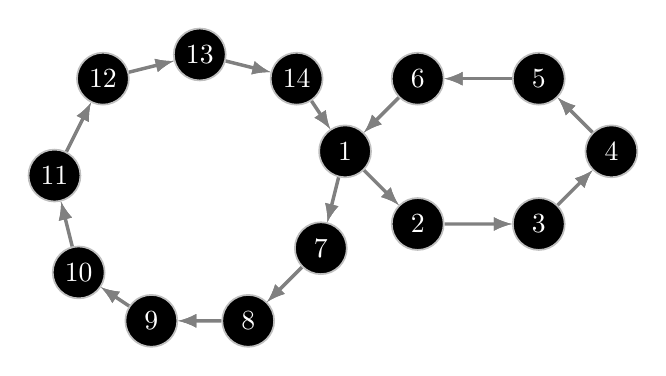
\begin{tikzpicture}[every node/.style={inner sep=0pt,white},
	scale=0.7,
	every edge/.style={
	draw,line width=1.25, ->, >=latex,color=gray,
        postaction={decorate,
                    decoration={markings,mark=at position 1 with {\arrow{>}}}
                   }
        }    
]%line width=1.25, ->, >=latex, 
\node (1) [circle, minimum size=18.75pt, fill=black, line width=0.625pt, draw=lightgray] at (212.5pt, -75.0pt) {1};
\node (2) [circle, minimum size=18.75pt, fill=black, line width=0.625pt, draw=lightgray] at (250.0pt, -112.5pt) {2};
\node (3) [circle, minimum size=18.75pt, fill=black, line width=0.625pt, draw=lightgray] at (312.5pt, -112.5pt) {3};
\node (7) [circle, minimum size=18.75pt, fill=black, line width=0.625pt, draw=lightgray] at (200.0pt, -125.0pt) {7};
\node (14) [circle, minimum size=18.75pt, fill=black, line width=0.625pt, draw=lightgray] at (187.5pt, -37.5pt) {14};
\node (13) [circle, minimum size=18.75pt, fill=black, line width=0.625pt, draw=lightgray] at (137.5pt, -25.0pt) {13};
\node (12) [circle, minimum size=18.75pt, fill=black, line width=0.625pt, draw=lightgray] at (87.5pt, -37.5pt) {12};
\node (11) [circle, minimum size=18.75pt, fill=black, line width=0.625pt, draw=lightgray] at (62.5pt, -87.5pt) {11};
\node (8) [circle, minimum size=18.75pt, fill=black, line width=0.625pt, draw=lightgray] at (162.5pt, -162.5pt) {8};
\node (9) [circle, minimum size=18.75pt, fill=black, line width=0.625pt, draw=lightgray] at (112.5pt, -162.5pt) {9};
\node (10) [circle, minimum size=18.75pt, fill=black, line width=0.625pt, draw=lightgray] at (75.0pt, -137.5pt) {10};
\node (6) [circle, minimum size=18.75pt, fill=black, line width=0.625pt, draw=lightgray] at (250.0pt, -37.5pt) {6};
\node (5) [circle, minimum size=18.75pt, fill=black, line width=0.625pt, draw=lightgray] at (312.5pt, -37.5pt) {5};
\node (4) [circle, minimum size=18.75pt, fill=black, line width=0.625pt, draw=lightgray] at (350.0pt, -75.0pt) {4};
\path 
(1) edge (2)
(2) edge (3)
(3) edge  (4)
(4) edge  (5) 
(5) edge  (6) 
(6) edge (1) 
(1) edge  (7) 
(7) edge  (8)
(8) edge  (9) 
(9) edge  (10)
(10) edge  (11)
(11) edge  (12)
(12) edge  (13) 
(13) edge  (14)
(14) edge  (1);
\end{tikzpicture}
\end{document}

